\begin{enumerate}
\item In \figref{fig:12.3}, if $P$ is $(2,4,5)$, find the coordinates of $F$.
\begin{figure}[h]
\centering
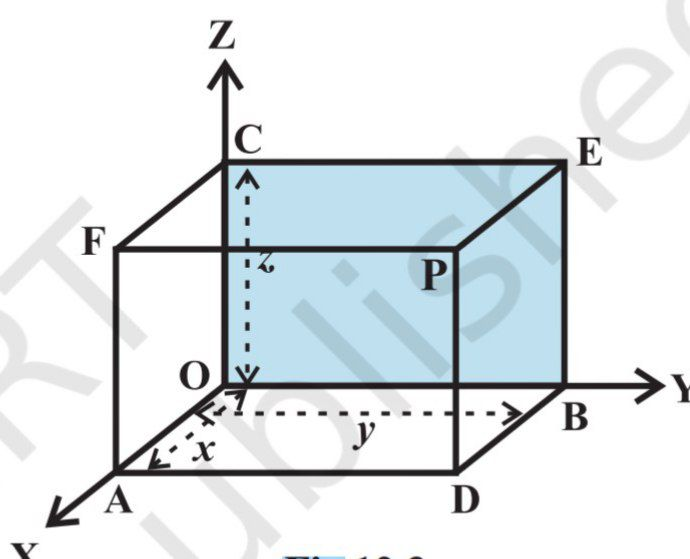
\includegraphics[width=\columnwidth]{chapters/11/figs/12.3.png}
\caption{12.3}
\label{fig:12.3}
\end{figure}
\item Find the octant in which the points $(-3,1,2)$ and $(-3,1,-2)$ lie.
\item Find the distance between the origin $O$ and any point $Q(x_2,y_2,z_2)$.
\item Show that the points $P(-2,3,5), Q(1,2,3)$ and $R(7,0,-1)$ are collinear. 
\item Are the points $A(3,6,9), B(10,20,30)$ and $C(24,-41,5)$ the vertices of a right angled triangle?
\item Find the equation of set of points $P$ such that $PA^2+PB^2=2k^2$, where $A$ and $B$ are the points $(3,4,5)$ and $(-1,3,-7)$, respectively.
\item Find the coordinates of the point which divides the line segment joining the points $(1,-2,3)$ and $(3,4,-5)$ in the ratio $2:3$
\begin{enumerate}[label=(\roman*)]
\item internally, and
\item externally
\end{enumerate}
\item Using section formula, prove that the three points $(-4,6,10), (2,4,6)$ and $(14,0,-2)$ are collinear.
\item Find the coordinates of the centroid of the triangle whose vertices are $(x_1,y_1,z_1), (x_2,y_2,z_2)$ and $(x_3,y_3,z_3)$.
\item Find the ratio in which the line segment joining the points $(4,8,10)$ and $(6,10,-8)$ is divided by the $YZ$- plane.
\item Show that the points $A(1,2,3), B(-1,-2,-1), C(2,3,2)$ and $D(4,7,6)$ are the vertices of a parallelogram $ABCD$, but it is not a rectangle.
\item Find the equation of the set of the points $P$ such that its distances from the points $A(3,4,-5)$ and $B(-2,1,4)$ are equal.
\item The centroid of a triangle $ABC$ is at the point $(1,1,1)$. If the coordinates of $A$ and $B$ are $(3,-5,7)$ and $(-1,7,-6)$, respectively find the coordinates of the point $C$.
\end{enumerate}

